\subsection{Contingent Claims}

\subsubsection{Pricing with Binomial Models}

\begin{remark} \hlt{One-Period Binomial Model}\\
At $t=1$, there are only two outcomes: up $u = \frac{S^+}{S}$ and down $d = \frac{S^-}{S}$, where $S^+, S^-$ are stock prices.\\
Let $h$ be number of units of underlying bought, $c^+$ and $c^-$ be value of call if underlying goes up or down.\\
Solve for the appropriate hedge ratio where $-c^+ + h S^+ = -c^- + hS^-$ (cash flow at $t=1$ is equal):
\begin{equation}
h = \frac{c^+ - c^-}{S^+ - S^-} \geq 0 \nonumber
\end{equation}
To either borrow or lend amount such that future net cash flows are  equal to zero. The cash flows are then\\
\begin{tabularx}{\textwidth}{p{14em}|p{14em}|X|X}
\hline
\rowcolor{gray!30}
Strategy & $t=0$ & $t=1$ Down & $t=1$ Up \\
\hline
$1$) Write one call option & $+c$ & $-c^-$ & $-c^+$ \\
$2$) Buy $h$ underlying units & $-hS$ & $+hS^-$ & $+hS^+$ \\
$3$) Borrow or lend & $-PV(-hS^- + c^-)$ & $-hS^- + c^-$ & $-hS^+ + c^+$ \\
& $= -PV(-hS^+ + c^+)$ & & \\
Net cash flow & $+c-hS - PV(-hS^- + c^-)$ & $0$ & $0$ \\
\hline
\end{tabularx}
The value of net portfolio at $t=0$ or else there is arbitrage opportunity. Hence,
\begin{align}
+c &-hS - PV(-hS^- + c^-) = +c-hS - PV(-hS^+ + c^+) = 0 \nonumber \\
c &= hS + PV(-hS^- + c^-) = hS + PV(-hS^+ + c^+)\nonumber
\end{align}
The financed amount is then $PV(-hS^- + c^-)=PV(-hS^+ + c^+)$; long call is equal to owning $h$ shares of stock partially financed. The no-arbitrage single-period put option valuation is then
\begin{align}
p &= hS + PV(-hS^- + p^-) = hS + PV(-hS^+ + p^+) \nonumber \\
h &= \frac{p^+ - p^-}{S^+ - S^-} \leq 0 \nonumber
\end{align}
To replicate long put, short underlying and lend portion of proceeds.
\end{remark}

\begin{method} \hlt{Expectations Approach to Binomial Model}\\
Results in identical value as no-arbitrage  approach, and is easier to compute.
\begin{align}
c &= PV[\pi c^+ + (1-\pi)c^-] \nonumber \\
p &= PV[\pi p^+ + (1-\pi)p^-] \nonumber \\
\pi &= \frac{FV(1)-d}{u-d}, \ \ \ FV(1) = \frac{1}{PV(1)} = 1+r \nonumber
\end{align}
The expected terminal option payoffs are then
\begin{align}
E(c_1) &= \pi c^+ + (1-\pi)c^- \nonumber \\
E(p_1) &= \pi p^+ + (1-\pi)p^- \nonumber
\end{align}
where $c_1$, $p_1$ are option value at $t=1$. Option values are then
\begin{align}
c &= PV_r[E(c_1)] \nonumber \\
p &= PV_r[E(p_1)] \nonumber
\end{align}
\end{method}

\begin{remark} \hlt{Put-Call Parity}\\
Value of put option may be determined based on put-call parity, where
\begin{equation}
S + p = PV(X) + c \nonumber 
\end{equation}
where $S$ is long stock, $p$ is long put, $PV(X)$ is present value of exercise price $X$.
\end{remark}

\begin{method} \hlt{Two-Period Binomial Method}\\
Valuation is similar to single period binomial model, except requiring more steps.
\begin{enumerate}[label=\roman*.]
\setlength{\itemsep}{0pt}
\item Calculate stock value at $t=2$
\item Calculate the option payoffs at $t=2$
\item Calculate expected option payoff using the up and down probabilities for $t=2$
\item Discount expected option payoff at $t=2$ back one period at risk-free rate to get option values at $t=1$
\item Calculate expected option value at end of $t=1$ using up and down probabilities
\item Discount expected option value at end of $t=1$ back one period at risk-free rate for option values at $t=0$
\end{enumerate}
\end{method}

\begin{remark} \hlt{Valuation of American-Style Options}\\
Early exercise feature not valuable for call options on non-dividend paying stocks.\\
Deep-in-the-money put options could benefit from early exercise, allowing capture of intrinsic value of the option and forgoing the time value. If intrinsic value may be invested at risk-free rate, interest earned is less than time value in most cases. The upside is limited as stock price $\geq 0$; interest on intrinsic value can exceed time value.\\
For valuation, same process as binomial model is used, except at each node, take maximum of exercise value and intrinsic value. For dividend-paying stocks, stock price falls when stock goes ex-dividend, hence to exercise the call option before such a decline in price.
\end{remark}

\begin{figure}[H]
\centering
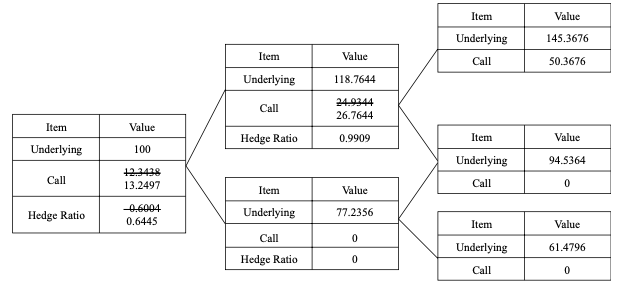
\includegraphics[scale=0.55]{/derivatives/americancallbinmodel}
\caption{Two-period binomial option for American-style call option with dividends}
\end{figure}

\begin{remark} \hlt{Valuation of Interest Rate Option with Binomial Tree}\\
Interest rate at each node is the one-period forward rate.\\
Call option has positive payoff when reference rate is greater than exercise rate,
\begin{equation}
\text{Call Payoff} = NA \times \max(0, \text{Reference Rate} - \text{Exercise Rate}) \nonumber
\end{equation}
Call options increase in value when rates increase.\\
Put option has positive payoff when reference rate is less than exercise rate,
\begin{equation}
\text{Put Payoff} = NA \times \max(0, \text{Exercise Rate} - \text{Reference Rate}) \nonumber
\end{equation}
Put option increases in value when rates decrease.\\
Valuation of options with binomial tree is similar to that of stock options, where value of each node is present vale of expected value of option. Model assumes that options cash settle at maturity.
\end{remark}

\subsubsection{Pricing with Black-Scholes-Merton (BSM) Models}

\begin{definition} \hlt{Black-Scholes-Merton (BSM) Model}\\
Values options in continuous time, based on no-arbitrage condition.\\
Main principle is to hedge the option by buying and selling underlying asset in a specific way to eliminate risk.
\end{definition}

\begin{remark} \hlt{Assumptions of BSM Model}
\begin{enumerate}[label=\roman*.]
\setlength{\itemsep}{0pt}
\item Underlying follows continuous Geometric Brownian Motion, $dS_t = \mu S_t + \sigma S_t d W_t$, $\mu$ is drift, $\sigma$ is volatility.
\item Underlying asset is liquid.
\item Short selling is permitted, with no market frictions and no arbitrage opportunities.
\item Options are European options.
\item Risk-free rate and volatility is known and constant. Borrowing and lending is at risk-free rate.
\end{enumerate}
\end{remark}

\begin{remark} \hlt{BSM Model Equation}
\begin{align}
c &= SN(d_1) - e^{-rT}XN(d_2) \nonumber \\
p &= e^{-rT}XN(-d_2) - SN(-d_1) \nonumber \\
d_1 &= \frac{\ln(S/X) + (r + \sigma^2/2)T}{\sigma T}, \ \ \ d_2 = d_1 - \sigma\sqrt{T} \nonumber
\end{align}
where $N(x)$ is standard normal cumulative distribution function.\\
Model provides the present value of expected option payoff at expiration.\\
Calls are replicated with long $N(d_1)$ units of stock, short $N(d_2)$ units of bonds with value of $e^{-rT}X$.\\
Puts are replicated with long $N(-d_2)$ units of bonds, short $N(-d_1)$ units of stock.\\
Note $N(d_2)$ is risk-neutral probability that call option will expire in the money, likewise $N(-d_2)$ for puts.
\end{remark}

\begin{flushleft}
Binomial Optino Pricing vs BSM
\begin{tabularx}{\textwidth}{p{11em}|X|X|X|X}
\hline
\rowcolor{gray!30}
Model & Call Underlying & Call Financing & Put Underlying & Put Financing \\
\hline
Binomial Model & $hS$ & $PV(-hS^- + c^-)$ & $hS$ & $PV(-hS^- + p^-)$ \\
BSM Model & $N(d_1)S$ & $-N(d_2) e^{-rT} X$ & $-N(-d_1)S$ & $N(-d_2) e^{-rT}X$ \\
\hline
\end{tabularx}
\end{flushleft}

\begin{remark} \hlt{BSM Model for Options on Stocks with Carry Benefits}
\begin{align}
c &= Se^{-\gamma T}N(d_1) - e^{-rT}XN(d_2) \nonumber \\
p &= e^{-rT}XN(-d_2) - Se^{-\gamma T}N(-d_1) \nonumber \\
d_1 &= \frac{\ln(S/X) + (r - \gamma + \sigma^2/2)T}{\sigma T}, \ \ \ d_2 = d_1 - \sigma\sqrt{T} \nonumber
\end{align}
where $\gamma$ is the carry benefits. Value of put option may be found based on carry-benefit adjusted put-call parity.
\begin{equation}
p + S e^{-\gamma T} = c + e^{-rT} X \nonumber
\end{equation}
\end{remark}

\begin{remark} \hlt{BSM Model for Options on Currencies}
\begin{align}
c &= Se^{-r(F)T}N(d_1) - e^{-r(B)T}XN(d_2) \nonumber \\
p &= e^{-r(B)T}XN(-d_2) - Se^{-r(F)T}N(-d_1) \nonumber \\
d_1 &= \frac{\ln(S/X) + (r(B) - r(F) + \sigma^2/2)T}{\sigma T}, \ \ \ d_2 = d_1 - \sigma\sqrt{T} \nonumber
\end{align}
where $r(F)$ and $r(B)$ is foreign and base risk-free interest rate.\\
The value of option may be thought of as having a bond component and a foreign exchange component.\\
The carry benefit is the interest earned on deposit of foreign currency.\\
Spot exchange rate $S$ is discounted at the base or foreign currency exchange rate, and bond component $e^{-r(B)T}X$ is the exercise exchange rate discounted at the base exchange rate.
\end{remark}

\begin{remark} \hlt{Black Model for Options on Futures}\\
Assume future prices follow Geometric Brownian Motion, ignoring margin requirements and mark-to-market.
\begin{align}
c &= e^{-rT}[F_0(T)N(d_1) - XN(d_2)] \nonumber \\
p &= e^{-rT}[XN(-d_2) - F_0(T)N(-d_1)] \nonumber \\
d_1 &= \frac{\ln[F_0(T)/X] + (\sigma^2/2)T}{\sigma \sqrt{T}}, \ \ \ d_2 = d_1 - \sigma\sqrt{T} \nonumber
\end{align}
where $F_0(T)$ is futures price at $t=0$ that expires at $t=T$, and $\sigma$ is volatility of futures price.\\
Model provides present value of difference between futures price and exercise price, adjusted by $N(\cdot)$.\\
Note, black model is just BSM model with $e^{-rT}F_0(T)$ substituted in place of $S$.\\
Calls are replicated with long $N(d_1)$ units of futures and short $N(d_2)$ units of bonds.\\
Puts are replicated with long $N(-d_2)$ units of bonds and short $N(-d_1)$ units of futures.
\end{remark}

\begin{remark} \hlt{Standard Market Model for Options on Forward Rate Agreements (FRAs)}\\
Call option on FRA gains when rates rise. Put option on FRA gains when rates fall. Interest rates on FRAs are fixed in advance, and settled in arrears. FRA uses $30/360$, but options on FRAs use $\text{Actual}/365$.\\
Value of option on notional capital of $1$ is:
\begin{align}
c &= (AP)e^{-r(t_{j-1} + t_m)}[FRA(0, t_{j-1}, t_m)N(d_1) - R_{X}N(d_2)] \nonumber \\
p &= (AP)e^{-r(t_{j-1} + t_m)}[R_{X}N(-d_2) - FRA(0, t_{j-1}, t_m)N(-d_1)] \nonumber \\
d_1 &= \frac{\ln[FRA(0, t_{j-1}, t_m)/R_X] + (\sigma^2/2)t_{j-1}}{\sigma \sqrt{t_{j-1}}}, \ \ \ d_2 = d_1 - \sigma\sqrt{T} \nonumber
\end{align}
where $AP=\text{Actual}/365$ is accrual period in years, $FRA(0, t_{j-1}, t_m)$ is fixed rate on FRA at $t=0$ which expires at $t = t_{j-1}$, with underling maturing at $t_j = t_{j-1} + t_m$, on an annual basis. $\sigma$ is annualised standard deviation.
\end{remark}

\begin{remark} \hlt{Replication of Contracts with Interest Rate Options}
\begin{enumerate}[label=\roman*.]
\setlength{\itemsep}{0pt}
\item Long interest rate call option and short interest rate put replicates a receive-floating, pay-fixed FRA.
\item If exercise rate $=$ current FRA rate, long interest rate put option and short interest rate call option is equivalent to receive-fixed, pay-floating FRA.
\item Set of floating-rate loan payments can be hedged with long position in an \hlt{interest rate cap} (portfolio or strip of interest rate call options (caplets)) encompassing a series of interest rate call options.
\item Floating-rate bond can be hedged with an \hlt{interest rate floor} (portfolio or strip of interest rate put options (floorlets)) encompassing a series of interest rate put options.
\item Long interest rate cap and short interest rate floor with exercise prices at swap rate is equivalent to a receive-floating, pay-fixed swap. If underlying is above strike, the cap and swap payoff to the party. If underlying is below strike, party must make payment on floor and swap.
\item Short interest rate cap and long interest rate floor can replicate a receiver swap.
\item If exercise rate $=$ swap rate, value of cap $=$ value of floor at the swap. When interest rate swap is initiated, current value zero (at-market swap). 
\item If exercise rate selected such that cap value $=$ floor value, then initial cost of long cap and short floor is also zero, which occurs when cap strike $=$ floor strike $=$ swap rate.
\end{enumerate}
\end{remark}

\begin{remark} \hlt{Swap Options (Swaption)}\\
Gives holder the right but not obligation to enter a swap at the pre-agreed swap rate.
\begin{enumerate}[label=\roman*.]
\setlength{\itemsep}{0pt}
\item Payer Swaption: option on a swap to pay-fixed, receive-floating. As interest rates rise, option becomes more valuable. Holder will exercise if market rate is greater than exercise rate at expiration.
\item Receiver Swaption: option to receive-fixed, pay-floating. As interest rates decrease, option becomes more valuable. Holder will exercise if market rate is less than exercise rate at expiration.
\end{enumerate}
Swaption is equivalent to option on series of cash flows, one for each settlement date of underlying swap, equal to difference between exercise rate and market swap fixed rate.
\end{remark}

\begin{remark} \hlt{Modified Black Model for Options on Swaps}\\
Let $AP$ be accrual period, $\sigma$ be volatility of forward swap rate.\\
PV of annuity matching forward swap payment is
\begin{equation}
\text{PVA} = \sum\limits_{j=1}^n PV_{0, t_j} (1) \nonumber
\end{equation}
The term is also referred to as an annuity discount factor. Model is then
\begin{align}
\text{PAY}_{\text{SWN}} &= (AP) \text{PVA} [r_{\text{Fix}} N(d_1) - r_{X} N(d_2)] \nonumber \\
\text{REC}_{\text{SWN}} &= (AP) \text{PVA} [r_{X} N(-d_2) - r_{\text{Fix}} N(-d_1)] \nonumber \\
d_1 &= \frac{\ln[r_{\text{Fix}}/r_X] + (\sigma^2/2)T}{\sigma \sqrt{T}}, \ \ \ d_2 = d_1 - \sigma\sqrt{T} \nonumber
\end{align}
where $r_{\text{Fix}}$ is market swap fixed rate, $r_X$ is exercise rate.\\
Actual premium to be scaled by notional amount.\\
Model requires adjustments: one for accrual period, and one for present value of annuity.\\
Note discount factor is absent, as present value of annuity embeds the option-related discount factor.\\
Underlying is a fixed rate on a forward interest rate swap.\\
Swaption may be described as present value of expected option payoff at expiration,
\begin{align}
\text{PAY}_{\text{SWN}} &= PV[E(\text{PAY}_{\text{SWN}, T})] = PV[e^{rT} \text{PAY}_{\text{SWN}}] \nonumber \\
\text{REC}_{\text{SWN}} &= PV[E(\text{REC}_{\text{SWN}, T})] = PV[e^{rT} \text{REC}_{\text{SWN}}] \nonumber
\end{align}
Payer is long swap with $r_{\text{Fix}}$ variable, short bond with $r_X$ variable. Vice versa for receiver.
\end{remark}

\begin{remark} \hlt{Replication of Swaptions}
\begin{enumerate}[label=\roman*.]
\setlength{\itemsep}{0pt}
\item Long receiver, short payer with same exercise rate replicates receive-fixed, pay-floating swap.
\item Long payer, short receiver with same exercise rate replicates pay-fixed, receive-floating swap.
\item If exercise rate of payer and receiver set such that values of payer and receiver are equal, then exercise rate is equal to market forward swap fixed rate.
\item Long straight fixed-rate bond and short receiver replicates callable fixed-rate bond.
\end{enumerate}
\end{remark}

\subsubsection{Option Greeks and Dynamic Hedging}

\begin{definition} \hlt{Delta}\\
Change in price of derivative instrument given a change in value of underlying.\\
Option delta for calls and puts are
\begin{align}
\bm{\Delta}_{\text{Call}} &= e^{-\delta T}N(d_1), \ \ \ \bm{\Delta}_{\text{Put}} = - e^{-\delta T}N(-d_1) \nonumber
\end{align}
where $\delta$ is dividend yield on the stock.
\end{definition}

\begin{remark} \hlt{Delta Change with Change in Price and Time}\\
As stock price increase, call option goes deeper in the money, and $N(d_1) \rightarrow 1$.\\
As stock price decrease, call option goes deeper out of money, and $N(d_1) \rightarrow 0$.\\
As $t \rightarrow T$, $\Delta \rightarrow 0$ if option is out of money, or $N(d_1) \rightarrow 1$ if option is in the money.
\end{remark}

\begin{definition} \hlt{Delta Hedging} \\
Establishing a position in underlying as prescribed by option delta so as to have no exposure to small movements in underlying price. Delta neutral portfolio is where portfolio delta is close to zero.\\
Let $N_H$ he number of units of option, $\bm{\Delta}_H$ be Delta of option. Delta neutral implies $\bm{\Delta}_{\text{Portfolio}} + N_H \bm{\Delta}_H = 0$.\\
Optimal number of hedging units is then
\begin{equation}
N_H = - \frac{\bm{\Delta}_{\text{Portfolio}}}{\bm{\Delta}_H} \nonumber
\end{equation}
Delta hedging is imperfect, and gets worse as underlying moves away from exercise price of hedging instrument.
\end{definition}

\begin{definition} \hlt{Gamma}\\
Change in derivative delta given change in underlying value.\\
Measures curvature of option price in relation to underlying price.
\begin{equation}
\Gamma_{\text{Call}} = \Gamma_{\text{Put}} = \frac{e^{-\delta T}}{S \sigma \sqrt{T}} n(d_1) \geq 0 \nonumber
\end{equation}
where $n(\cdot)$ is the standard normal probability density function.
\end{definition}

\begin{remark} \hlt{Gamma Change with Change in Price and Time}\\
Gamma has largest value for at-the-money options.\\
Deep in-the-money or deep out-of-money options have low gamma.\\
Gamma changes with stock price changes and with time to expiration.\\
Call and put options on same underlying asset with same exercise price, time-to-expiration have equal gammas.
\end{remark}

\begin{definition} \hlt{Gamma Neutral Portfolio}\\
To decrease (increase) gamma of portfolio, to short (long) options.\\
Once revised portfolio has reached desired gamma, may then get portfolio level to desired level as step two, by either buying or selling stock (positive delta, zero gamma).
\end{definition}

\begin{remark} \hlt{Gamma Risk}\\
If assumptions of BSM hold, changes in stock price will be continuous, hence there will be no gamma risk.\\
Gamma risk is the risk that stock price might abruptly jump, leaving the delta-hedged portfolio unhedged.\\
A delta-hedged portfolio that is long stocks and short calls will have negative net gamma exposure.
\end{remark}

\begin{remark} \hlt{Change in Option Price Approximation with Delta and Gamma}\\
Change in option price may be approximated with Delta and Gamma as follows:
\begin{align}
\Delta c = \bm{\Delta}_{\text{Call}} \times \Delta S + \frac{1}{2} \Gamma \times (\Delta S)^2, \ \ \ \Delta p = \bm{\Delta}_{\text{Put}} \times \Delta S + \frac{1}{2} \Gamma \times (\Delta S)^2 \nonumber
\end{align}
where $\bm{\Delta}$ is Delta; $\Delta$ is change in $(\cdot)$; $c, p, S$ are call, put, and stock prices.
\end{remark}

\begin{figure}[H]
\centering
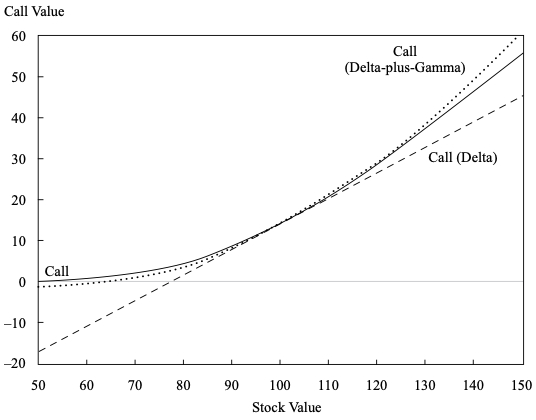
\includegraphics[scale=0.33]{/derivatives/deltagamma}
\caption{Call option Delta $\bm{\Delta}$ and Gamma $\Gamma$}
\end{figure}

\begin{definition} \hlt{Theta (Time Decay)}\\
Change in option price to passage of time. Speed of option value decline $\uparrow$ as $t \rightarrow T$.\\
As time passes, option's speculative value declines, all else equal. Note, $\Theta \leq 0$, and $\Theta \rightarrow 0$ as $t \rightarrow T$.
\end{definition}

\begin{definition} \hlt{Vega}\\
Change in option price to changes in volatility of returns on underlying.\\
Vega of call equals Vega of put, based on put-call parity. As options are at or near the money, $\mathcal{V} \uparrow$.\\
Futures and options on various volatility indexes may be used to manage Vega exposure.
\end{definition}

\begin{definition} \hlt{Rho}\\
Change in option price to changes in risk-free rate.\\
Rho of call is positive, as buying an option avoids financing costs with purchasing the stock. $i/r \uparrow \rightarrow c \uparrow$.\\
Rho of put is negative, as selling the stock delays opportunity to earn interest on proceeds from sale. $i/r \uparrow \rightarrow p \downarrow$.
\end{definition}

\begin{figure}[H]
\centering
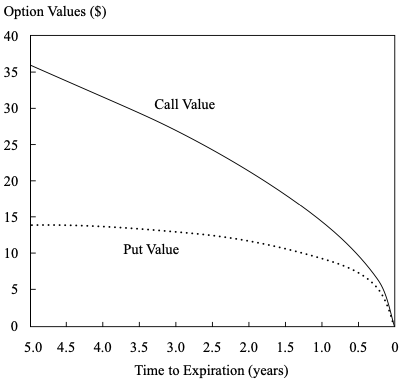
\includegraphics[scale=0.35]{/derivatives/theta}
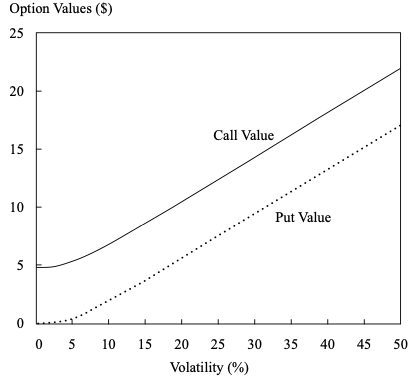
\includegraphics[scale=0.35]{/derivatives/vega}
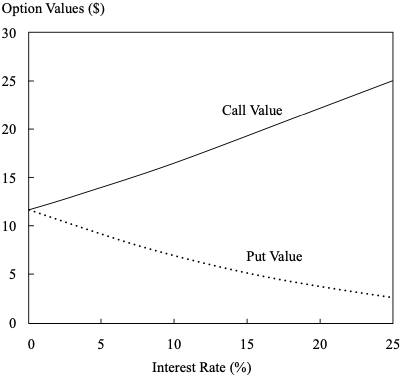
\includegraphics[scale=0.35]{/derivatives/rho}
\caption{Option Theta $\Theta$, Vega $\mathcal{V}$ and Rho $\rho$}
\end{figure}

\begin{remark} \hlt{Implied Volatility}\\
Standard deviation of continuously compounded asset returns as implied by market price of an option.\\
To get implied volatility, input stock price, exercise price, risk-free rate, time-to-maturity into BSM model.\\
Different implied volatilities for different exercise prices and for calls and puts with same terms are observed.\\
Term structure of volatility is the plot of implied volatility with respect to time-to-expiration.\\
Volatility smile is the plot of implied volatility with respect to exercise price.\\
Volatility surface is the combined plot of term structure and volatility smile; flat if BSM assumptions are true.\\
Implied volatility may be used to gauge market perception. Options with same underlying with different exercise prices may have different implied volatility, violating BSM assumption of constant volatility.\\
Implied volatility may be used to quote option prices. Options with different exercise prices and maturity dates may be quoted using same unit of measurement.
\end{remark}